\section{Final Design}
The final design of the robot's drive system is very similar to the proposed design provided to Penguin ASI and Laurentian University in December. Using a belt drive over a chain drive was accepted through our proposal along with keeping it battery powered. In the final design the batteries used were ones that were provided by Penguin ASI. Four batteries were still required to power all four brushless DC motors and two other batteries required to supply power to the other electronic components on board the robot. The final design also had features that were in the proposed design, such as removable interior components, easy serviceability and keeping it as a modular design. Having the components easily removable will allow anyone who is maintaining the drive system have access to all the bearings for re-greasing and easy vision for inspection of belts condition.  After assembling one exterior drive box, some small design changes were made that were not noticed in the CAD model assemblies or were notified to us from Penguin Employees after the proposal report had been submitted. None of these changes required the proposed design to drastically change but actually improved the overall design and reduced the amount of machining time required for some components. An example of reducing machining time would be the new hubs located at the back side do the drive boxes. In the proposed design the rear hubs required machining on both the exterior and interior, but with the new design all exterior machining was not required. Table~\ref{tab:specs} gives general robots specifications.

\begin{table}[htbp]
\centering
\caption{Robot Specifications}
\begin{tabular}{| p{5cm}ll |} \hline
Component & Value & Unit \\ \hline
Total Mass & 1385.99 & kg \\
Top Speed & 3	& km/h \\
Total power & 2,982.8 & W \\
Location of centre of mass (height off ground) & 0.477 & m\\ \hline
 \end{tabular}
 \label{tab:specs}
 \end{table}

The exploded view of assembly that can be seen in Figure~\ref{fig:quart_assem} shows how each individual drive box goes together along with its connection to the robots frame. All four motors sit inside the robot frame and are each coupled with a flexible Lovejoy coupling to the output shaft that rotates within the pivot. The torque from the motor is then transferred through the output shaft and is then transmitted through the belt to two wheel shafts. Those wheel shafts each have a foam filled tire attached to the end with a tapered fit mount and a castle nut ensuring the mount doesn't come off the tapered shaft mount.

\begin{figure}[htbp]
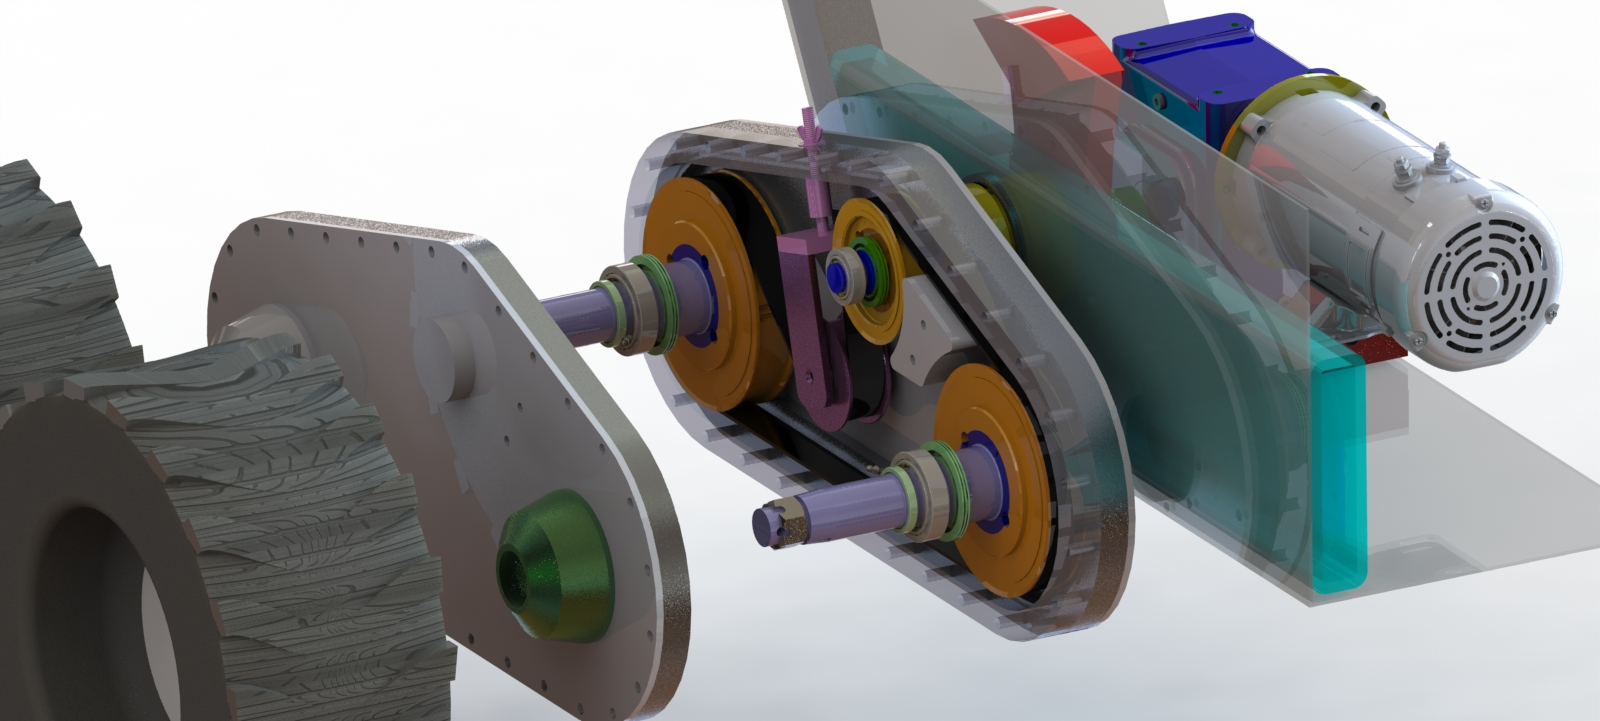
\includegraphics[width=\linewidth]{images/drive_box_presentation_rndr.jpg}
\caption[Quarter view of robot]{Rendering showing one quarter of robot exterior drive assembly with front case frame and wheels off. }
\label{fig:quart_assem}
\end{figure}

What makes this design a more acceptable design over the previous design that Penguin ASI originally had is the simplicity of it. In their previous design their was only two motors used to power the four ex trier drive boxes, which required that two output shafts on one side had to share the output from one motor. In the new design each drive box will be getting its own motor to provide power and this reduces the amount of moving parts needed. Such as a chain to allow each output shaft to be sharing one motor and tensions along that chain. Each component added raises a new point of possible failure during operation, so reducing the amount of moving parts also decreases this possibility. Another feature that the new design has over the old is the accessibility of the components inside the drive box for maintenance and repair if required. The new design gives you full access to all the interior components once the front case plate is removed. From this,  the wheel shafts and the output shaft are easily removed, only a set screw at the coupling is needs to be loosened. All moving components can now be accessed easily and reduces the time required for an individual to work on. Using belts over chains reduces the maintenance cost, since belts do not require any lubrication and run in a dry casing.


